\section{Resultados e discussão}
\noindent Neste capítulo são apresentados os resultados obtidos sobre o potencial de balanço energético nulo e quase nulo para as edificações propostas. No primeiro momento, os modelos foram classificados segundo a classe de eficiência energética disposta pelo INI-C, seguidos das otimizações que resultaram na análise de impacto das medidas implementadas. Após as otimizações foram avaliados os sistemas de produção de energia solar fotovoltaica propostos, e a capacidade de geração de energia anual.\vspace*{0.3cm} \newline
\noindent Verificou-se que a otimização e as estratégias ativas e passivas proporcionaram as condições necessárias para o balanço energético dos modelos. Ao final das simulações de consumo e produção de energia, foi analisada a viabilidade econômica das soluções propostas. Esta análise mostrou condições econômicas favoráveis de implantação do sistema de produção de energia proposto aos modelos.  Estes dados foram expressos em gráficos e tabelas a fim de facilitar a compreensão dos resultados alcançados.
\subsection{Classificação de desempenho energético dos modelos genéricos}
\noindent Para a determinação da classe de eficiência energética dos modelos genéricos, segundo a metodologia descrita pelo INI-C, é exigida a comparação entre dois cenários definidos como modelo real e o modelo de referência. Desta forma, foram configurados os cenários para a identificação do consumo total de energia térmica, elétrica e de energia primária, como descrito no capítulo 3. Como resultado, foi constatada a baixa eficiência energética dos modelos, como exposto na Tabela \ref{tab:tabela15}.
\begin{table}[H]
    \centering
    \small
    \caption{Resultados da classificação de desempenho energético dos modelos genéricos iniciais.}
\begin{tabular}{llll}
    \hline
    \textbf{Descrição}                                    & \textbf{Variável}      & \makecell[c]{\textbf{Modelo} \\\textbf{Real}} & \makecell[c]{\textbf{Modelo de} \\\textbf{Referência}}  \\ \hline
    \multicolumn{4}{c}{\textbf{Classe de desempenho energético - modelo de 8 pavimentos}}                                                  \\ \hline
    \makecell[l]{Consumo total de \\energia térmica}                      & CTEt (kWh/ano)         & 418197               & 443178                         \\
    \makecell[l]{Consumo total de \\energia elétrica - CTEe}              & CTEe (kWh/ano)         & 1086401              & 1142584                        \\
    \makecell[l]{Consumo de energia primária \\da edificação selecionada} & \makecell[l]{CEP real/ref \\(kWh/ano)} & 2198258,3            & 2315630,2                      \\ \hline
    \multicolumn{3}{l}{Etiqueta da edificação real}                                                       & \multicolumn{1}{c}{\textbf{D}} \\ \hline
    \multicolumn{4}{c}{\textbf{Classe de desempenho energético - modelo de 19 pavimentos}}                                                 \\ \hline
    \makecell[l]{Consumo total de \\energia térmica}                      & CTEt (kWh/ano)         & 1115708              & 1137261                        \\
    \makecell[l]{Consumo total de \\energia elétrica - CTEe}              & CTEe (kWh/ano)         & 2643097              & 2676556                        \\
    \makecell[l]{Consumo de energia primária \\da edificação selecionada} & \makecell[l]{CEP real/ref \\(kWh/ano)} & 5456234              & 5533476,7                      \\ \hline
    \multicolumn{3}{l}{Etiqueta da edificação real}                                                       & \multicolumn{1}{c}{\textbf{D}} \\ \hline
    \end{tabular}
    \begin{flushleft}
        \par \small \vspace{0.1cm} Fonte: autor (2019).
    \end{flushleft}
    \label{tab:tabela15}
\end{table}
\noindent O desempenho enérgico dos modelos ampara a necessidade de otimização, quanto as características construtivas e de sistemas das edificações, para tornar as condições de performance propícias ao balanço energético.
\subsection{Impacto das variáveis sobre o consumo anual de energia elétrica}
\noindent A etapa de otimização possibilitou visualizar a influência das variáveis sobre o consumo anual final das edificações para cada cenário definido. Os resultados da implementação das medidas ativas de redução de consumo de energia, disponíveis nos Apêndices deste trabalho, demonstraram maior peso entre as variáveis de estratégia ativa, pertencentes aos blocos de simulação 2, 3 e 9, e passivas, formadas pelos blocos de simulação 1, e de 4 a 10, como exposto nos Gráficos 4 e 5.\vspace*{0.3cm} \newline
\noindent Nota-se que as variáveis de estratégias ativas reduziram significativamente o consumo anual, com curvas de queda expressivas, direcionando a média de consumo para baixo, posicionando alguns cenários abaixo da média linear, como observado entre os blocos de simulação 1 ao 7 do Gráfico 4. Este comportamento se estende até o bloco de simulação 7 no modelo de 19 pavimentos, desempenho demonstrado no Gráfico 5. Os blocos de simulação compostos por variáveis passivas apresentaram constância de forma e estreitamento ao longo do avanço das implementações das medidas. O estreitamento gradativo da amplitude da curva de consumo final anual em ambos os resultados sugere que o avanço cumulativo das medidas de mitigação de consumo é importante para o sucesso do processo de adequação da edificação ao conceito \textit{Zero Energy}.\vspace*{0.3cm} \newline
\noindent A tendência ascendente das curvas de consumo, a partir do bloco de simulação 4, é causada pela alteração do PAF\textsubscript{T}, partindo da menor razão, de 30\%, até alcançar a maior razão entre área de fachada e área de aberturas envidraçadas, com 80\%. Esta medida aponta a importância da adoção de aberturas menores, em torno de 30\%, para a melhor relação entre o PAF\textsubscript{T} e o consumo energético da edificação.\vspace*{0.3cm} \newline
\noindent Os gráficos serviram como instrumento de tomada de decisão acerca da seleção dos melhores cenários para a etapa de simulação de geração de energia solar fotovoltaica. Além disso, os gráficos facilitaram a visualização da importância de cada estratégia adotada para o balanço energético nulo das edificações avaliadas. A leitura dos gráficos pode ser feita da seguinte forma:
\begin{itemize}
    \item Os gráficos consistem em evidenciar o impacto das medidas adotadas no consumo da edificação. Para tal, foi definida a comparação entre o desempenho dos modelos por meio do percentual de redução de consumo de energia entre as edificações. Esta comparação desconsidera a escala dos gráficos, já que ambos correspondem a edificações de portes diferentes, e considera o comportamento das medidas aplicadas por meio de análise das curvas de consumo;
    \item Os pontos na cor laranja representam cada cenário montado, os quais variam entre 4 conjuntos de implementação sequencial de medidas de redução de energia. Cada conjunto de cenários pertencentes aos 10 blocos de simulação estão definidos e representados nos Gráficos 4 e 5;
    \item As curvas em verde representam a tendência de aumento ou redução de consumo de 
    energia entre a simulação dos cenários;
    \item Como a mudança entre os tipos de vidro avaliados, foi necessário realizar novas simulações de todos os blocos anteriores a esta medida, sendo essa etapa representada pelas curvas acentuadas entre conjuntos de cenários, como, por exemplo, observado na curva entre os cenários 12 e 13 do bloco de simulação 10, na página 93.            
\end{itemize}
\noindent A redução de consumo provocada pela implementação de equipamentos e iluminação mais eficientes atinge o patamar de 22,48\% de redução global, assim como o sistema de arrefecimento, com 34,78\% para o modelo de 19 pavimentos. As reduções no modelo de 8 pavimentos foram tênues, da ordem de 16,09 e 16,66\%, respectivamente, para os sistemas de arrefecimento, e equipamentos e iluminação, como observado na Figura 21.\vspace*{0.3cm} \newline
\noindent Entretanto, cabe mencionar que o desempenho de controle térmico do sistema Split para o modelo de 19 pavimentos, nos cenários iniciais, provocou maior consumo de energia em relação aos dois outros sistemas de arrefecimento avaliados, CAG e VRF, em 22,73\%. Após a implementação do vidro mais eficiente, houve redução do consumo em cerca de 24,91\%, superando ligeiramente em performance o sistema CAG. Em contraste a esta observação do Split para o modelo de 19 pavimentos, este sistema obteve comportamento semelhante ao sistema VRF para a edificação de 8 pavimentos, com considerável performance e redução de consumo de energia. O \textit{Split} apresentou controle satisfatório das médias de temperatura de conforto das zonas térmicas. A diferença de desempenho dos sistemas de condicionamento de ar entre os dois modelos pode ser atribuída a diferença de carga térmica entre as edificações, onde o modelo de 8 pavimentos apresenta menor carga térmica e menor exposição à radiação solar em comparação ao modelo de 19 pavimentos.\vspace*{0.3cm} \newline
\begin{figure}[H]
    \centering
    \rotatebox{90}{
        \begin{minipage}{\textheight}
            \caption{Consumo \textit{versus} medidas do modelo genérico de 8 pavimentos.}
            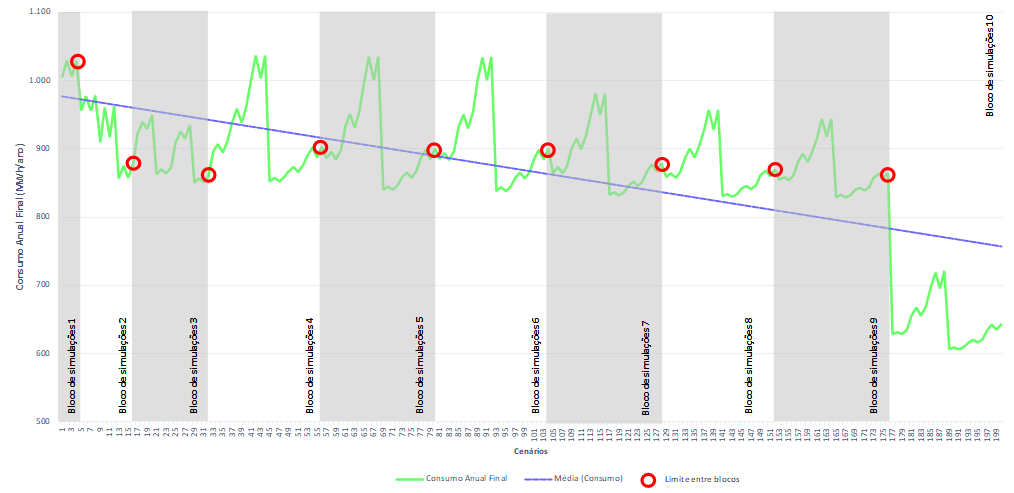
\includegraphics[width=1.0\textwidth]{figures/result/fig23-grafico4.png}
            \begin{flushleft}
                \par \small Fonte: autor, (2020). Legenda: Bloco de simulações 1 a 3 – Blocos com implementação do vidro, orientações solares e sistemas de condicionamento de ar; Bloco de simulações 4 –Bloco com implementação das variações de PAF\textsubscript{T}; Bloco de simulações 5 e 6 – Blocos com implementação de paredes e coberturas; Bloco de simulações 7 e 8 e 9 – Blocos com implementação das proteções solares; Bloco de simulações 10 – Blocos com implementação das medidas de redução de carga.
            \end{flushleft}
            \label{fig:figure23}
        \end{minipage}
    }
\end{figure}
\pagebreak

\begin{figure}[H]
    \centering
    \rotatebox{90}{
        \begin{minipage}{\textheight}
            \caption{Consumo \textit{versus} medidas do modelo genérico de 19 pavimentos.}
            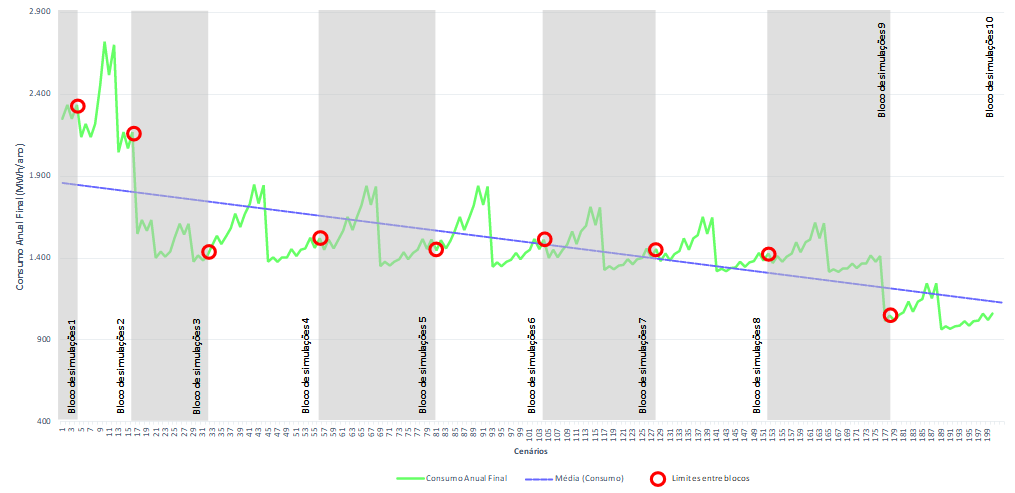
\includegraphics[width=1.0\textwidth]{figures/result/fig24-grafico5.png}
            \begin{flushleft}
                \par \small Fonte: autor, (2020). Legenda: Bloco de simulações 1 a 3 – Blocos com implementação do vidro, orientações solares e sistemas de condicionamento de ar; Bloco de simulações 4 –Bloco com implementação das variações de PAF\textsubscript{T}; Bloco de simulações 5 e 6 – Blocos com implementação de paredes e coberturas; Bloco de simulações 7 e 8 e 9 – Blocos com implementação das proteções solares; Bloco de simulações 10 – Blocos com implementação das medidas de redução de carga.
            \end{flushleft}
            \label{fig:figure24}
        \end{minipage}
    }
\end{figure}
\pagebreak
\noindent Como os vidros foram utilizados em todos os cenários, a importância da variável se torna mais visível quando comparado com todas as variáveis, assim como apresentado na Figura \ref{fig:figure25}. Verifica-se que, ao longo das implementações de medidas passivas, a influência é reduzida de 14,40\% para 4,00\%, conforme observado anteriormente nos blocos de simulação 3 e 4.\vspace*{0.3cm} \newline
\noindent Em ambos os resultados foi notado que a implementação de componentes construtivos com menor transmitância térmica acentua a diferença os cenários entre os modelos otimizados e os não-otimizados. Estes resultados retratam a importância das estratégias ativas para a redução do consumo total anual.
\begin{figure}[H]
    \centering
    \caption{Gráfico dos blocos de simulação das variáveis de vidro, orientação solar e do sistemas de condicionamento de ar e medidas de redução de carga dos modelos genérico de 8 (esq.) e 19 pavimentos (dir.)}
    \begin{subfigure}[b]{0.49\textwidth}
        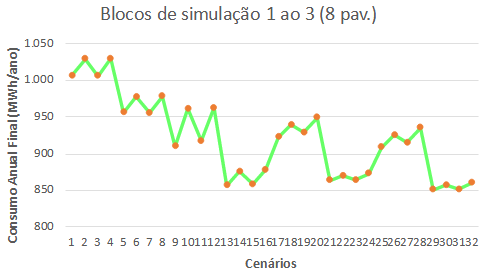
\includegraphics[width=\textwidth]{figures/result/fig25-bloco1-3.png}
    \end{subfigure}
    \begin{subfigure}[b]{0.49\textwidth}
        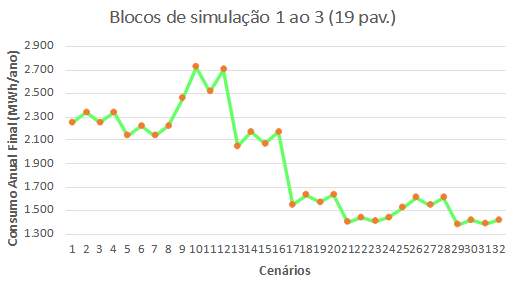
\includegraphics[width=\textwidth]{figures/result/fig26-bloco1-3.png}
    \end{subfigure}
    \begin{subfigure}[b]{0.49\textwidth}
        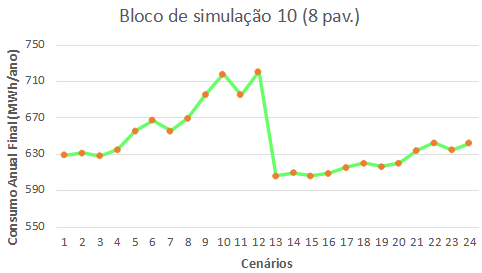
\includegraphics[width=\textwidth]{figures/result/fig27-bloco10.png}
    \end{subfigure}
    \begin{subfigure}[b]{0.49\textwidth}
        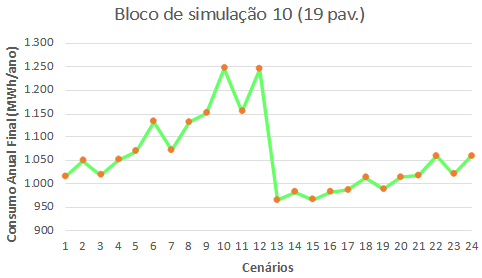
\includegraphics[width=\textwidth]{figures/result/fig28-bloco10.png}
    \end{subfigure}
    \begin{flushleft}
        \par \small Fonte: autor, (2020).
    \end{flushleft}
    \label{fig:figure25}
\end{figure}
\noindent As características das paredes e cobertura, blocos de simulação 5 e 6 respectivamente, na Figura 22, quando observadas isoladamente, são medidas importantes na redução de consumo, que neste caso representam 20\%, entre os componentes construtivos observados in loco e os componentes mais eficientes propostos para comparação. É verificada a suavização da curva de consumo entre o segundo conjunto de simulações, retratado pelos cenários 13 a 24, em relação ao primeiro conjunto, de 1 a 12, o que sinaliza a importância da envoltória e da redução da ação da radiação solar sobre os ambientes internos da edificação. A escala de consumo entre as edificações é acentuada nestes cenários, dada a semelhança do comportamento das curvas, porém, com amplitudes de 50 MW para o modelo de 8 pavimentos, e quase 200 MW para o modelo de 19 pavimentos.\vspace*{0.3cm} \newline
\noindent A influência destes componentes sobre o consumo final, junto ao vidro com baixa emissividade, atinge  o  patamar  de  26,72\%  para  a  análise  do  resultado  isolado,  como  exposto  na  Figura  \ref{fig:figure26}. Verifica-se, também, que as mudanças provocadas pela implementação das estratégias passivas, ao  longo  do  processo  de  otimização,  reduzem  a  relevância  do  vidro  com  menor  transmitância térmica para a composição construtiva e performance energética dos modelos.
\begin{figure}[H]
    \centering
    \caption{Gráficos dos blocos de simulação de paredes, 3, e coberturas, 4, dos modelos genéricos de 8 (esq.) e 19 pavimentos (dir.).}
    \begin{subfigure}[b]{0.49\textwidth}
        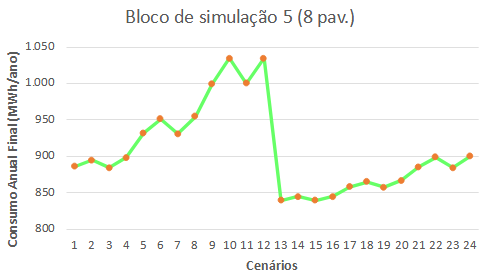
\includegraphics[width=\textwidth]{figures/result/fig29-bloco5.png}
    \end{subfigure}
    \begin{subfigure}[b]{0.49\textwidth}
        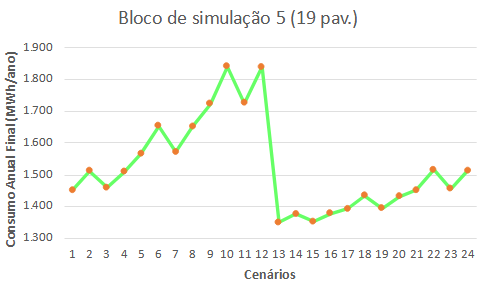
\includegraphics[width=\textwidth]{figures/result/fig30-bloco5.png}
    \end{subfigure}
    \begin{subfigure}[b]{0.49\textwidth}
        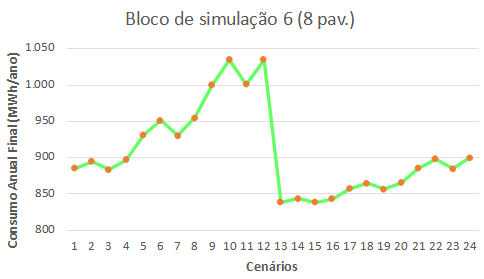
\includegraphics[width=\textwidth]{figures/result/fig31-bloco6.png}
    \end{subfigure}
    \begin{subfigure}[b]{0.49\textwidth}
        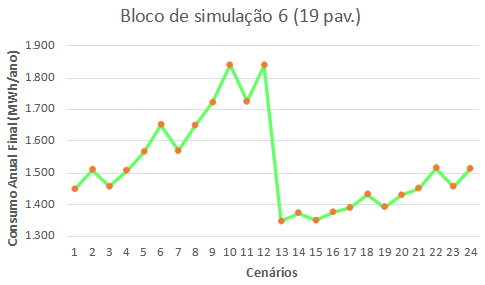
\includegraphics[width=\textwidth]{figures/result/fig32-bloco6.png}
    \end{subfigure}
    \begin{flushleft}
        \par \small Fonte: autor, (2020).
    \end{flushleft}
    \label{fig:figure26}
\end{figure}
\noindent As alterações sobre as variáveis do Percentual de Área de Abertura da Fachada Total, presentes na Figura \ref{fig:figure27}, representaram pouco impacto sobre o consumo final total quando comparado com as outras medidas implementadas. Entretanto, cabe citar que esta variável, quando observada isoladamente, corresponde a mesma grandeza de redução de consumo que as variáveis de componentes construtivos, reduzindo o consumo nos cenários simulados em cerca 18,95\% e 26,71\% para as edificações de 8 e 19 pavimentos, respectivamente. 
\begin{figure}[H]
    \centering
    \caption{Gráficos dos blocos de simulação de PAF\textsubscript{T} dos modelos genérico de 8 (esq.) e 19 pavimentos (dir.).}
    \begin{subfigure}[b]{0.49\textwidth}
        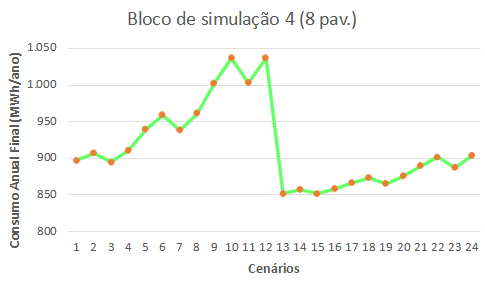
\includegraphics[width=\textwidth]{figures/result/fig33-bloco4.png}
    \end{subfigure}
    \begin{subfigure}[b]{0.49\textwidth}
        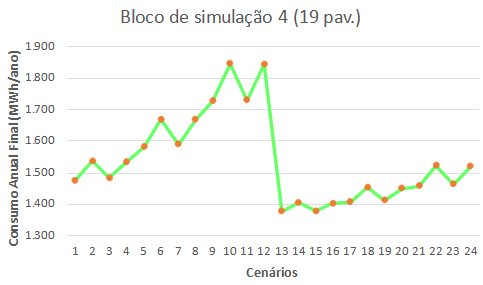
\includegraphics[width=\textwidth]{figures/result/fig34-bloco4.png}
    \end{subfigure}
    \begin{flushleft}
        \par \small Fonte: autor, (2020).
    \end{flushleft}
    \label{fig:figure27}
\end{figure}
A implementação das proteções solares, Figura \ref{fig:figure28}, apresentou redução de 6,96\% sobre o consumo total entre os blocos de simulação 5 e 6. Além desta redução, nota-se o estreitamento entre os cenários 12 e 13 neste bloco, em 23,52\%, reduzindo em 3,19\% a em relação aos blocos anteriores. Nota-se também a suavização da curva nos cenários 13 a 24 em ambas as simulações do modelo de 8 pavimentos, o que sugere a influência sobre o consumo ao controlar a quantidade de luz e de radiação no ambiente, por meio da implantação de proteções solares e de vidros mais eficientes.
\begin{figure}[H]
    \centering
    \caption{Bloco de simulações de protetores solares dos modelos genérico de 8 (esq.) e 19 pavimentos (dir.).}
    \begin{subfigure}[b]{0.49\textwidth}
        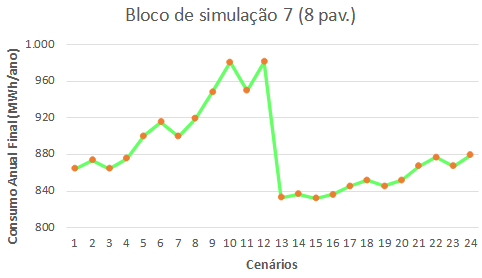
\includegraphics[width=\textwidth]{figures/result/fig35-bloco7.png}
    \end{subfigure}
    \begin{subfigure}[b]{0.49\textwidth}
        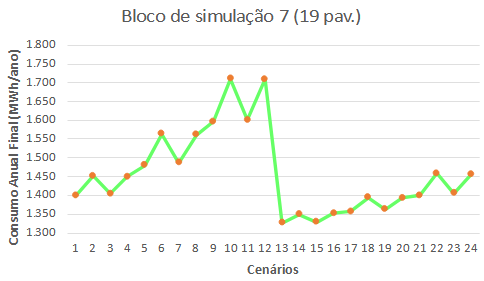
\includegraphics[width=\textwidth]{figures/result/fig36-bloco7.png}
    \end{subfigure}
    \begin{subfigure}[b]{0.49\textwidth}
        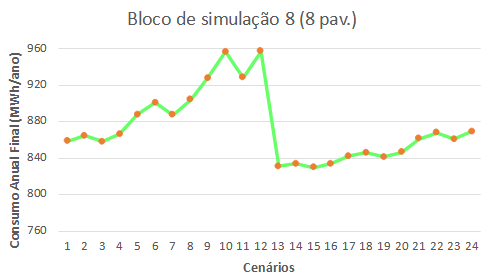
\includegraphics[width=\textwidth]{figures/result/fig37-bloco8.png}
    \end{subfigure}
    \begin{subfigure}[b]{0.49\textwidth}
        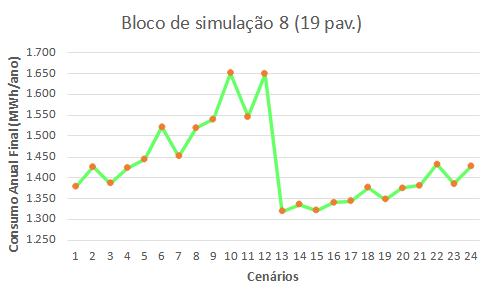
\includegraphics[width=\textwidth]{figures/result/fig38-bloco8.png}
    \end{subfigure}
    \begin{subfigure}[b]{0.49\textwidth}
        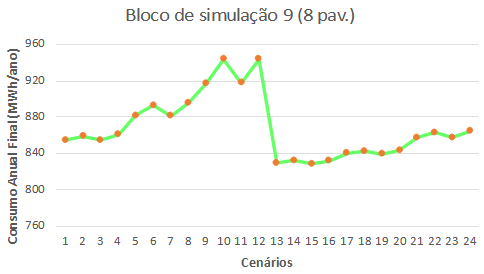
\includegraphics[width=\textwidth]{figures/result/fig39-bloco9.png}
    \end{subfigure}
    \begin{subfigure}[b]{0.49\textwidth}
        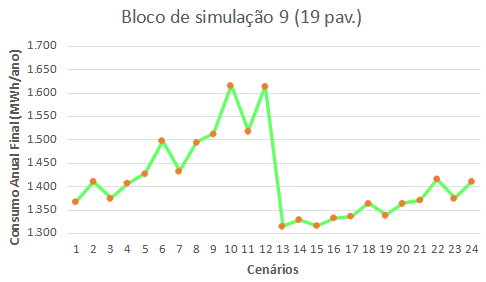
\includegraphics[width=\textwidth]{figures/result/fig40-bloco9.png}
    \end{subfigure}
    \begin{flushleft}
        \par \small Fonte: autor, (2020).
    \end{flushleft}
    \label{fig:figure28}
\end{figure}
\subsection{Geração de energia solar fotovoltaica}
\noindent Os modelos genéricos mais eficientes reduziram globalmente o consumo de energia elétrica, quando comparados com os modelos sem otimização, em cerca de 39,76\% para o modelo genérico otimizado mais eficiente, de 8 pavimentos, e 57,07\% para o modelo genérico otimizado mais eficiente, de 19 pavimentos. A partir destes resultados, foram selecionados os modelos mais eficientes entre os cenários simulados para cada tipologia e foram simuladas a implementação dos sistemas de produção de energia solar fotovoltaica.\vspace*{0.3cm} \newline
\noindent Observa-se que a energia elétrica gerada ao longo do ano, supriu a demanda de energia da edificação de 8 pavimentos para metade do ano e ligeiramente igualado em dois meses, abril e junho, como demonstrado no Gráfico 7. Anualmente, esta diferença é reduzida, produzindo maior energia do que a demanda anual, atingindo o balanço energético nulo, como apresentado no Gráfico 9. Nota-se, também, a proporção dos sistemas de condicionamento de ar – HVAC, iluminação e equipamentos em relação à produção de energia, correspondendo entre 30 a 40\% da composição do consumo para cada sistema avaliado. Os resultados com as configurações detalhadas dos equipamentos especificados estão descritos no Anexo I e II deste trabalho.
\begin{figure}[H]
    \centering
    \caption{Sistemas, consumo e produção de energia elétrica do modelo genérico de 8 pavimentos.}
    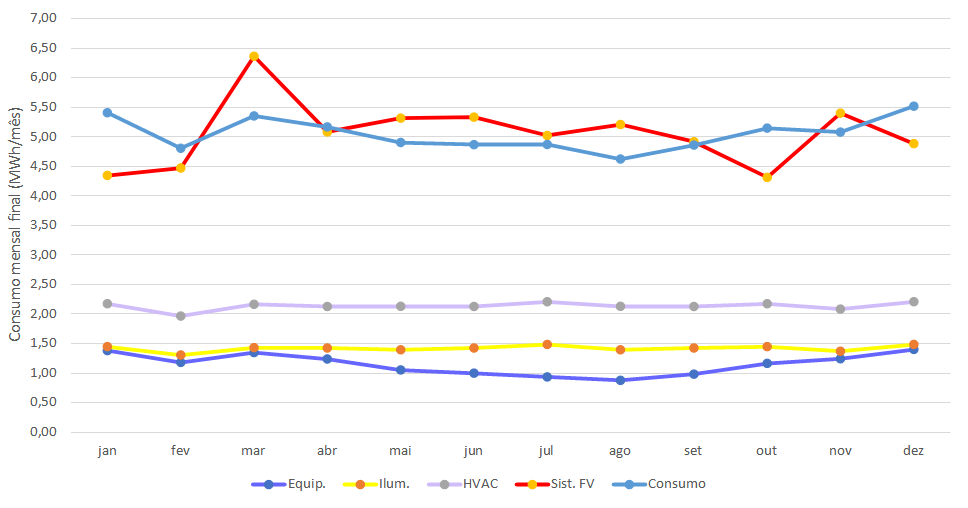
\includegraphics[width=1.0\textwidth]{figures/result/fig41-consumomod.png}
    \begin{flushleft}
        \par \small Fonte: autor, (2020).
    \end{flushleft}
    \label{fig:figure29}
\end{figure}
\noindent O desempenho do sistema de produção de energia fotovoltaica do modelo de 19 pavimentos atendeu à demanda anual. Nos meses de outubro e janeiro a demanda não foi correspondida, sendo quase nula a relação entre demanda e produção em dezembro, como observado no Gráfico 8. Observa-se que a proporção dos sistemas percebida no modelo de 8 pavimentos, em relação à produção de energia, é similarmente constatada neste modelo de 19 pavimentos.\vspace*{0.3cm} \newline
\noindent Os resultados de produção de energia para este modelo evidenciaram as características mais importantes para proporcionar maior geração de energia, como a área de fachada exposta a radiação solar e a relação entre a quantidade de pavimentos e a área de piso da edificação. Estes resultados de produção de energia em relação ao consumo foram importantes para indicar a potencialidade das edificações com dimensões como o modelo genérico proposto.
\begin{figure}[H]
    \centering
    \caption{Sistemas, consumo e produção de energia elétrica do modelo genérico de 19 pavimentos.}
    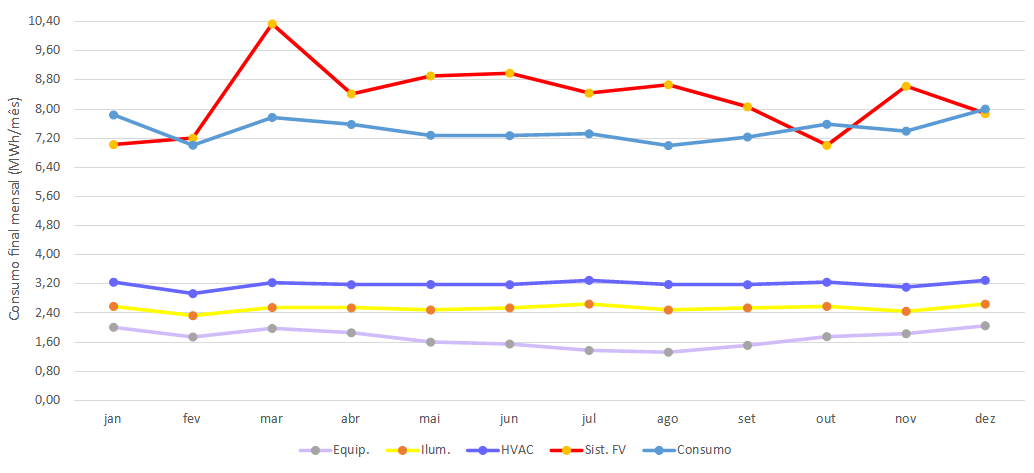
\includegraphics[width=1.0\textwidth]{figures/result/fig42-consumomod.png}
    \begin{flushleft}
        \par \small Fonte: autor, (2020).
    \end{flushleft}
    \label{fig:figure30}
\end{figure}
\vspace{-0.5cm} \noindent No Gráfico 9 e 14 são dispostas as médias mensais de consumo e produção de energia dos modelos genéricos otimizados de 8 e 19 pavimentos, respectivamente, assim como as médias anuais, as curvas tracejadas de média de produção de energia solar fotovoltaica e seus desvios padrões máximos e mínimos. Verificam-se os limites do sistema fotovoltaico para o modelo de 8 pavimentos, onde a relação quase nula entre geração e consumo de energia mensal é notada ao longo do ano simulado. Esta relação representa uma média anual de produção de energia superior ao consumo em 1,02\%, o que atesta o estado \textit{Zero Energy} para o modelo avaliado. Entretanto, a curva de desvio padrão mínimo mostra que em um cenário de pouca produção, o modelo seria dependente da energia fornecida pela concessionaria para atender as demandas mensais.\vspace{-0.3cm} 
\begin{figure}[H]
    \centering
    \caption{Consumo final mensal, Consumo vs. Produção de energia e Desvio Padrão das médias de produção de energia do modelo genérico otimizado de 8 pavimentos.}
    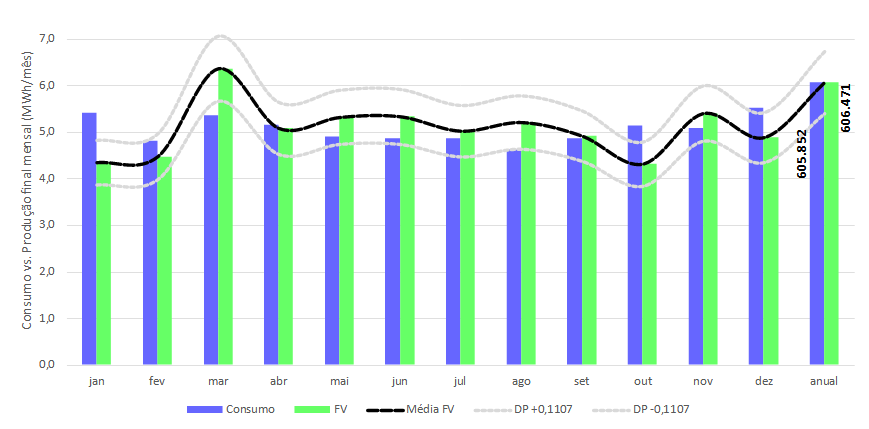
\includegraphics[width=1.0\textwidth]{figures/result/fig43-consumofinal.png}
    \begin{flushleft}
        \par \small Fonte: autor, (2020).
    \end{flushleft}
    \label{fig:figure31}
\end{figure}
\noindent Entretanto, para o cenário ótimo simulado para o modelo genérico otimizado de 19 pavimentos, percebe-se que não há a mesma dependência da Rede Pública para o fornecimento de energia. Este fato é constatado em um cenário onde a curva de desvio padrão mínimo seja a média de produção de energia do sistema sugerido, apresentando resultados superiores ao consumo na maior parte do ano.
\begin{figure}[H]
    \centering
    \caption{Consumo final mensal, Consumo vs. Produção de energia e Desvio Padrão das médias de produção de energia do modelo genérico otimizado de 19 pavimentos.}
    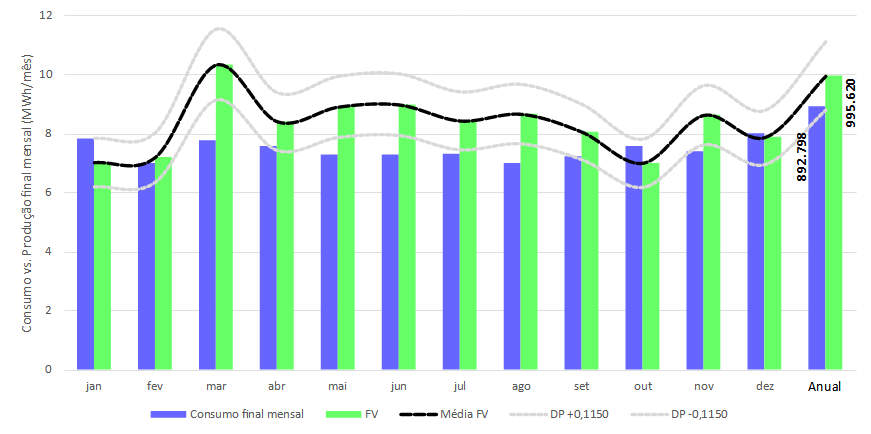
\includegraphics[width=1.0\textwidth]{figures/result/fig44-consumofinal.png}
    \begin{flushleft}
        \par \small Fonte: autor, (2020).
    \end{flushleft}
    \label{fig:figure32}
\end{figure}
\subsection{Análise de viabilidade econômica}
\noindent Os dados tarifários necessários para o cálculo de Custo Anual de Energia, CAE, foram elaborados conforme a atualização da concessionaria para o mês de janeiro de 2020. A edificação proposta é classificada como comercial e está alocada no subgrupo B3, modalidade tarifária convencional. Para o mês estudado, foi atribuído à Tarifa de Energia, TE, um acréscimo proveniente da bandeira amarela vigente. As Tarifas de Uso de Sistema de Distribuição, TUSD, e os impostos fiscais ICMS, PIS e COFINS para o período estão demonstrados na Tabela \ref{a}.
\begin{table}[H]
    \centering
    \small
    \caption{Tarifas e impostos para a modalidade tarifária convencional.}
    \begin{tabular}{ll}
    \hline
        \textbf{Tarifas e impostos}     &   \textbf{Valor}  \\\hline
        TE + Bandeira amarela           &   0,26484         \\
        TUSD                            &   0,27440         \\
        ICMS                            &   25\%            \\
        PIS+CONFINS                     &   1,57\%          \\\hline
    \end{tabular}
    \begin{flushleft}
        \par \small Fonte: autor, (2020).
    \end{flushleft}
    \label{a}
\end{table}
\noindent Para o cálculo de custo anual de energia, levou-se em consideração o consumo anual dos modelos otimizados de 8 e 19 pavimentos mais eficientes energeticamente, sendo 605.853 kWh/ano e 965.186 kWh/ano, seus respectivos consumos anuais de energia. Na Equação \ref{eq:eq11} é estabelecido o custo anual de energia sem impostos, considerando TE e TUSD.
\begin{align}\label{eq:eq11}
    &Custo_{8pav}=E_{consumida} \times (TE+TSUD)\nonumber \\
    &Custo_{8pav}=605.853 \times (0,26484+0,27440)\nonumber \\
    &Custo_{8pav}=326.700,17 \text{ reais}\nonumber \\
    &Custo_{19pav}=E_{consumida} \times (TE+TSUD)\nonumber \\
    &Custo_{19pav}=965.186 \times (0,26484+0,27440)\nonumber \\
    &Custo_{19pav}=520.166,89 \text{ reais}
\end{align}
\noindent Entretanto, os custos sofrem tributação de impostos pela distribuidora de energia, o que foi considerado para a composição real do custo anual de energia, como definido pela EDP e apresentado na Equação \ref{eq:eq12}.
\begin{align}\label{eq:eq12}
    &Custo_{8pav}=\frac{Custo_{s/imposto}}{1-(PIS+COFINS+ICMS)} \nonumber \\
    &Custo_{8pav}=\frac{326.700,17}{1-0,2675}\nonumber \\
    &Custo_{8pav}=444.913,75 \text{ reais}\nonumber \\
    &Custo_{19pav}=\frac{Custo_{s/imposto}}{1-(PIS+COFINS+ICMS)} \nonumber \\
    &Custo_{19pav}=\frac{520.166,89}{1-0,2675}\nonumber \\ 
    &Custo_{19pav}=708.384,70 \text{ reais}
\end{align}
\noindent Na Tabela \ref{tab:17} são apresentadas a quantidade de energia gerada no ano, assim como os custos dos sistemas de geração de energia solar fotovoltaica indicados, sendo que o custo de instalação por kWp dos sistemas foi orçado, em janeiro de 2020, em 784 reais para o filme fino Cd-Te \cite{Sorgato2018} e 3.682 reais para o sistema mono-Si sugerido, segundo a média de preço do mercado local.\newline
\begin{table}[H]
    \centering
    \caption{Produção de energia e custo de implantação dos sistemas fotovoltaicos.}
    \begin{tabular}{llll}
        \hline
        \multicolumn{4}{c}{\textbf{Modelo genérico de 8 pavimentos}}                                                                                                                                                                                                                \\ 
        \hline
        \textbf{Características}                                                        & \makecell[l]{\textbf{Cobertura e}\\ \textbf{estacionamento}}      & \makecell[l]{\textbf{Proteção}\\ \textbf{Solar}}          & \textbf{Fachada}                                          \\ 
        \hline
        Módulo                                                                          & \makecell[l]{SunPower \\SPR-E20-\\435-COM}                        & \makecell[l]{SunPower \\SPR-E20-\\435-COM}                & \makecell[l]{First Solar \\FS-4122-2}                     \\
        Inversor                                                                        & \makecell[l]{Fronius \\International \\IG Plus 150 V-3}           & \makecell[l]{Fronius \\International \\ECO 25.0-3-S}      & \makecell[l]{Fronius \\International \\IG Plus 150 V-3}   \\
        \makecell[l]{Energia gerada\\ (MWh/ano)}                                        & 236,40                                                            & 154,42                                                    & 215,65                                                    \\ 
        \hline
        \makecell[l]{Custo total por \\potência instalada (R\$)}                        & 552.300,00                                                        & 371.587,44                                                & 214.988,48                                                \\ 
        \hline
        \multicolumn{3}{l}{\makecell[l]{Energia total \\gerada (MWh/ano)}}                                                                                  & 606,47                                                                                                                \\
        \multicolumn{3}{l}{\makecell[l]{Custo total dos \\sistemas instalados (R\$)}}                                                                       & 1.138.875,92                                                                                                          \\ 
        \hline
        \multicolumn{4}{c}{\textbf{Modelo genérico de 19 pavimentos}}                                                                                                        \\
        \hline
        \textbf{Características}                                                        & \makecell[l]{\textbf{Cobertura e}\\ \textbf{estacionamento}}      & \textbf{Proteção Solar}                                   & \textbf{Fachada}                                          \\ 
        \hline
        Módulo                                                                          & \makecell[l]{SunPower \\SPR-E20-\\435-COM}                        & \makecell[l]{SunPower \\SPR-E20-\\435-COM}                & \makecell[l]{First Solar \\FS-4122-2}                     \\
        Inversor                                                                        & \makecell[l]{Fronius \\International \\ECO 27.0-3-S}              & \makecell[l]{Fronius \\International \\IG Plus 120 V-3}   & \makecell[l]{Fronius \\International \\IG Plus 150 V-3}   \\
        \makecell[l]{Energia gerada\\ (MWh/ano)}                                        & 236,40                                                            & 370,02                                                    & 397,12                                                    \\ 
        \hline
        \makecell[l]{Custo total por \\potência instalada (R\$)}                        & 552.300,00                                                        & 896.198,80                                                & 376.084,80                                                \\ 
        \hline
        \multicolumn{3}{l}{\makecell[l]{Energia total \\gerada (MWh/ano)}}                                                                                  & 1003,54                                                                                                               \\
        \multicolumn{3}{l}{\makecell[l]{Custo total dos \\sistemas instalados (R\$)}}                                                                       & 1.824.583,60                                                                                                          \\
        \hline
    \end{tabular}
    \begin{flushleft}
        \par \small Fonte: autor, (2020).
    \end{flushleft}
\end{table}
\noindent Os valores de retorno, V\textsubscript{r}, dos custos de implementação dos sistemas foram calculados com base na taxa de atratividade Selic de 4,5\% para o período de janeiro de 2020, representada pela incógnita i. Além disso, foram utilizados o custo anual de energia, A, e a vida útil especificada pela fabricante dos módulos utilizados, de 25 anos, representada pela incógnita \textit{n}.\newline
\begin{align}
    &V_{ret8pav}=444.913,75 \times \left\{\frac{1-\left[\frac{1}{(1+0,045)^25}\right]}{0,045}\right\} \nonumber \\
    &V_{ret8pav}=6.597.274,05 \text{ reais} \nonumber \\
    &V_{ret19pav}=708.384,70 \times \left\{\frac{1-\left[\frac{1}{(1+0,045)^25}\right]}{0,045}\right\} \nonumber \\
    &V_{ret19pav}=10.504.070,01 \text{ reais} \nonumber
\end{align}
\noindent O valor de retorno calculado dos investimentos é utilizado para estipular o valor presente, VP, de cada um dos sistemas propostos.
\begin{align}
    &V_{8pav}=6.597.274,05 - 1.138.875,92 = 5.458.398,13 \nonumber \\
    &V_{19pav}=10.504.070,01 - 1.824.583,60 = 8.679.486,41 \nonumber
\end{align}
\noindent Assim, constata-se que os sistemas de produção de energia propostos aos modelos genéricos são economicamente viáveis, visto que os VP’s são positivos. Da mesma forma, o \textit{payback} da implantação dos sistemas estudados é de 2,55 anos para o modelo de 8 pavimentos e 2,57 anos para o modelo de 19 pavimentos. Vale mencionar que as variações das taxas de energia e a perda de eficiência do sistema ao longo da vida útil não foram consideradas na avaliação de viabilidade econômica \cite{Sorgato2018}.\vspace*{0.3cm} \newline
\noindent Os resultados indicam, para o modelo de edificação adotado, a teórica viabilidade de utilização do conceito \textit{Zero Energy} para as edificações comerciais de escritório de pequeno, médio e grande porte para o recorte territorial utilizado. As condições climáticas e urbanas favoráveis, juntamente a adoção de materiais e componentes adequados ao cenário brasileiro, priorizando soluções que proporcionaram a máxima extração dos recursos energéticos on site foram essenciais para alcançar o balanço energético nulo.